\section{Experiment 9I: fleet-informed active identification}
\label{sec:experiment9i}

\paragraph{Question and protocol.}
Experiment 9H shows that shared knowledge protects an information-limited new
client. Experiment 9I asks whether the fleet can also tell that client which
data to acquire next. Ten fresh fleets (seeds 186--195) use a mature 180-client
cohort to learn three latent groups and rank-two personalized backbones. Thirty
unseen clients each receive three initial 0.25~s records and exactly one 0.5~s
follow-up maneuver.

The frozen candidate library contains low-, medium-, and high-speed maneuvers at
0.22 and 0.50~Hz. Selection uses predicted Fisher information based on the
current estimate and nominal closed-loop input templates; realized candidate
outputs and evaluation trajectories are unavailable to every deployable policy.
Parameter-active policies minimize normalized parameter or coefficient
covariance. Control-active policies minimize covariance weighted by scheduled-
gain sensitivity. Local policies fit all three parameters; fleet policies use
the learned rank-two backbone. Fixed policies use the medium-speed, low-frequency
maneuver. Oracle-best-fleet tries all realized candidate records and minimizes
true scheduled-gain error; it is an unattainable diagnostic, not an oracle for
tracking itself.

The predeclared aggregate gate requires Fleet-control-active to improve both
Fleet-fixed and Local-control-active. This gate is accompanied by a mechanistic
check: a meaningful personalized active policy should not collapse to one
universal maneuver or become identical to its parameter-only ablation.

\begin{table}[htbp]
\centering
\caption{Experiment 9I equal-budget active-identification results.}
\label{tab:experiment9i-results}
\begin{tabular}{lrrr}
\toprule
Method & Tracking & Parameter error & Gain error\\
\midrule
Local fixed & 0.006846 & 0.0518 & 0.00445\\
Local parameter-active & 0.006843 & 0.0508 & 0.00439\\
Local control-active & 0.006736 & 0.0577 & 0.00376\\
Fleet fixed & 0.006857 & 0.0477 & 0.00443\\
Fleet parameter-active & 0.006724 & 0.0466 & 0.00351\\
Fleet control-active & 0.006724 & 0.0466 & 0.00351\\
Oracle gain selector & 0.006735 & 0.0397 & 0.00184\\
\bottomrule
\end{tabular}
\end{table}

\begin{figure}[htbp]
\centering
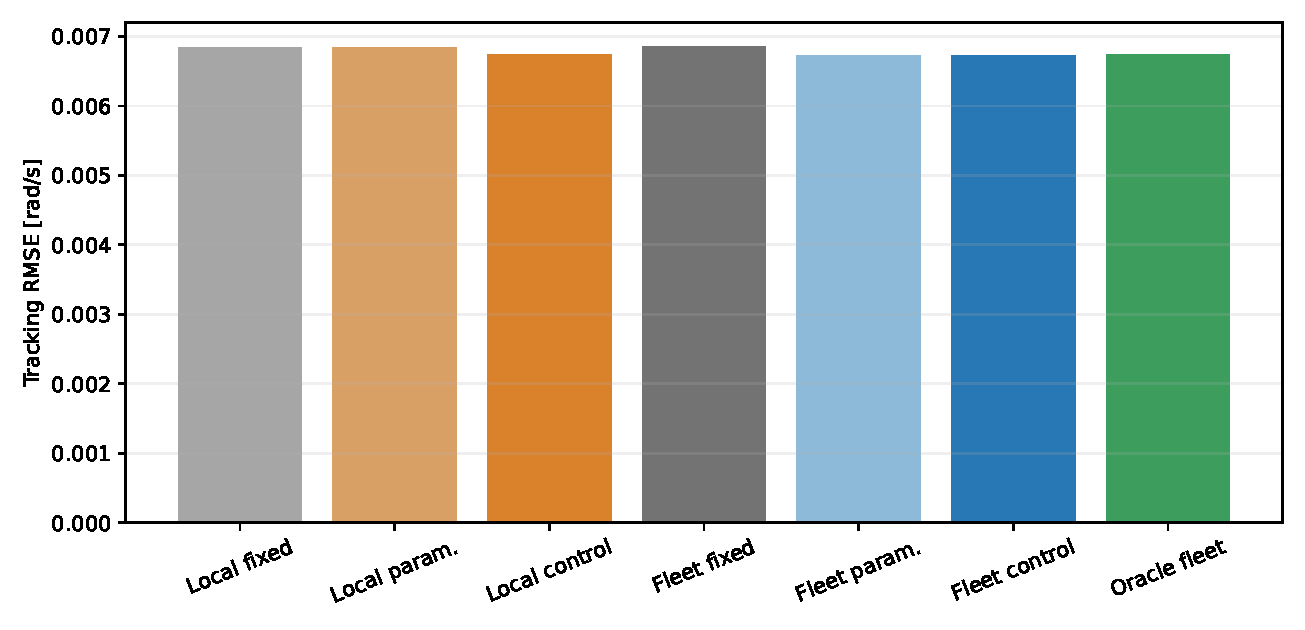
\includegraphics[width=0.84\linewidth]{../results/figures/experiment_9i_active_identification.pdf}
\caption{Tracking after one equal-duration follow-up maneuver. Active excitation
helps, but the tested fleet criteria collapse to the same universal choice.}
\label{fig:experiment9i}
\end{figure}

\paragraph{Aggregate result.}
Fleet-control-active improves Fleet-fixed by 1.94\% and Local-fixed by 1.78\%,
so it passes the literal aggregate gate. Local-control-active already improves
Local-fixed by 1.60\%. Consequently, the incremental fleet advantage over an
active Local client is only 0.18\% on average. It wins that paired comparison in
five of ten fleets; the fleet-wise difference ranges from 0.93\% better to
1.02\% worse. This is parity, not a reliable federated advantage.

The mechanism check is negative. Fleet-parameter-active and Fleet-control-active
select the high-speed, high-frequency maneuver for all 300 clients and produce
identical results. Local-control-active also makes that universal selection.
Thus the candidate library contains one maneuver that dominates both predicted
information criteria. The improvement over the deliberately fixed comparator
demonstrates the value of more informative excitation, but not individualized
fleet-informed experiment selection or control-aware weighting.

The oracle gain-error selector chooses all six candidates: high-fast for 77
clients, high-slow for 69, medium-fast for 47, medium-slow for 56, low-fast for
23, and low-slow for 28. This confirms that client-dependent best maneuvers exist
under the oracle gain metric. However, the local linearized criteria do not
predict that diversity. The oracle selector also need not minimize nonlinear
tracking, which explains why its aggregate tracking is slightly worse than the
universal high-fast fleet policy despite much lower gain error.

The server selects three groups with mean training ARI 0.998. All 3900 fits
converge, and all 6300 nonlinear evaluations remain feasible. Clustering,
optimization failure, and unsafe candidate maneuvers therefore do not explain
the collapse.

\paragraph{Decision.}
Experiment 9I does not justify pivoting the paper toward active learning in its
current form. The literal gate is too weak: it rewards discovering that one
globally informative maneuver is better than the fixed comparator. A genuine
federation-specific active result would need heterogeneous admissible maneuver
sets, operating conditions, or excitation costs, together with a posterior
criterion capable of predicting client-dependent value. Adding those elements
now would substantially broaden the IEEE IV paper and risk appearing designed
to manufacture differentiation.

The recommended paper core therefore remains the empirically supported result
from 9H: shared group backbones and progressive personalization protect cold-
start clients, while sufficiently informed Local models catch up. Active
experiment selection may be retained as a transparent negative boundary or
developed later as a separate contribution. The immediate next requirement for
the current paper is an explicit distributed implementation of shared-backbone
learning, including partial participation and communication accounting, followed
by a frozen confirmation. Privacy can then be integrated into the shared updates
while keeping personalization coefficients local.

\paragraph{Reproducibility.}
The protocol is frozen in \path{code/config/experiment_9i.json}; the implementation
is \path{code/experiments/experiment_9i_active_identification.py}. Aggregate and
seed-level results, selected-maneuver counts, diagnostics, and provenance hashes
are stored under \path{results/tables}.
